\section{Top Tagging}
\label{sec:toptagging}

When a jet is boosted, the substructure can be exploited for tagging. Taggers apply criteria meant to separate signal jets from background. Machine Learning can also be applied to improve tagging abilities. In this analysis, the DeepAK8 mass decorrelated tagger is used. DeepAK8 is a machine learning tagger that takes a list of particle information and a list of secondary vertex information as inputs. The lists are then processed separately by 1 dimensional convolutional neural networks, then the outputs of the two separate layers are used as inputs in a fully connected layer, shown in Figure~\ref{fig:deepak8}.

Since many particle features are correlated with mass, the CNN is able to extract the mass of the jets. In some cases, a tagger needs to be independent of the mass of the jet. In this analysis, the background estimate uses the softdrop mass as an input, and so a tagger that does not bias the mass distribution is needed.

DeepAK8 has a mass decorrelated version which is developed by adding and additional mass prediction neural network. This mass prediction network calculates the accuracy of the CNN do extract the mass of the jet, and penalizes the tagger when the accuracy his high. 


\begin{figure}[h]
\centering
	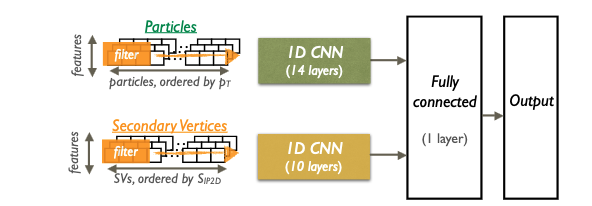
\includegraphics[width=0.8\textwidth]{figures/deepak8.png}
	\caption{Diagram of the DeepAK8 neural network.}
	\label{fig:deepak8}
\end{figure}